\documentclass[10pt,xcolor={svgnames}]{beamer}

%%%%% Colors
\usetheme{Dresden}%\usetheme{Madrid}
\colorlet{beamer@blendedblue}{green!55!black}
%%%%%

%%%%% Other 
\addtobeamertemplate{navigation symbols}{}{%
    \usebeamerfont{footline}%
    \usebeamercolor[fg]{footline}%
    \hspace{1em}%
    \insertframenumber/\inserttotalframenumber
}
\usepackage{hyperref, url}

\definecolor{pine_green}{HTML}{007935}
\hypersetup{colorlinks,breaklinks,linkcolor=white,urlcolor=orange,citecolor=black}
\renewcommand\thefootnote{\textcolor{pine_green}{\arabic{footnote}}}
\usepackage{cancel}
%%%%%

%%%%% Greying out/invidible Slides
\setbeamercovered{invisible}
\setbeamercovered{%
  again covered={\opaqueness<1->{15}}}
  
%%%%%







%%%%% Footnotes and captions
%\usepackage[utf8]{inputenc}
\usepackage{caption}
\usepackage{comment}
\usepackage{wasysym}
\setbeamerfont{footnote}{size=\tiny}
\setbeamerfont{caption}{size=\tiny}
%\setbeamerfont{normal text}{size=\small}
\setbeamerfont{itemize/enumerate body}{size=\small}
\setbeamerfont{itemize/enumerate subbody}{size=\footnotesize}
%%%%%



%Information to be included in the title page:
\title[Connor Wiegand]{Intro to Economic Analysis: Microeconomics}
\subtitle{EC 201 - Day 2 Slides}
\author[EC 201]{Connor Wiegand}
\institute[]{Department of Economics - University of Oregon}
\date{29 September 2021}


\begin{document}

\frame{\titlepage}

\begin{frame}{Back to Our Model}
    \begin{itemize}[<+->]
        \item So suppose there are two goods in our economy: guns and butter
        \item Suppose that we have finite resources, some which are used to make both guns and butter (e.g. labor) 
        \item Consider a table outlining some combinations of guns and butter that we can produce:
        \begin{table}[H]
            \centering
            \begin{tabular}{c|c}
                Guns & Butter  \\
                \hline
                60 & 0\\
                50 & 18\\
                40 & 28\\
                30 & 35\\
                20 & 42\\
                10 & 47\\
                0 & 50\\
            \end{tabular}
        \end{table}
        \item Observations?
    \end{itemize}
\end{frame}


\begin{frame}{Observations}

\end{frame}


\begin{frame}{What if we tried to graph this?}
\pause
\vspace{62mm}
\begin{itemize}
    \item This is called a \textit{Production Possibilities Frontier}
\end{itemize}
\end{frame}


\begin{frame}{PPF}
\begin{itemize}[<+->]
    \item A \underline{\textbf{Production Possibilities Frontier}} is a graph that shows the various combinations of output that an economy can produce using it's resources and technology
    \item An outcome \footnote{i.e., an example of such a combination of outputs} is said to be \textit{efficient} if it is \underline{on} the production possibilities frontier
    \item An outcome is said to be \textit{inefficient} if it is inside the PPF
    \item An outcome is said to be \textit{unattainable} if it is outside the PPF
\end{itemize}
\end{frame}

\begin{frame}{Example}
\begin{itemize}[<+->]
    \item A \underline{\textbf{Production Possibilities Frontier}} is a graph that shows the various combinations of output that an economy can produce using it's resources and technology
    \item An outcome \footnote{i.e., an example of such a combination of outputs} is said to be \textit{efficient} if it is \underline{on} the production possibilities frontier
    \item An outcome is said to be \textit{inefficient} if it is inside the PPF
    \item An outcome is said to be \textit{unattainable} if it is outside the PPF
\end{itemize}
\end{frame}

\begin{frame}{The Regions of a PPF}
\begin{itemize}[<+->]
    \item A \underline{\textbf{Production Possibilities Frontier}} is a graph that shows the various combinations of output that an economy can produce using it's resources and technology
    \item An outcome \footnote{i.e., an example of such a combination of outputs} is said to be \textit{efficient} if it is \underline{on} the production possibilities frontier
    \item An outcome is said to be \textit{inefficient} if it is inside the PPF
    \item An outcome is said to be \textit{unattainable} if it is outside the PPF
\end{itemize}
\end{frame}


\begin{frame}{Example}

\end{frame}

\begin{frame}{The Shape of a PPF}
\begin{itemize}[<+->]
    \item Consider the following production possibilities set\footnote{I will refer to a list of points on the PPF as a production possibilities set. I reality, a production possibilities set would just be \textit{all} the points on a PPF curve}:
    \begin{table}[]
        \centering
        \begin{tabular}{|c|ccccccccccc|}
        \hline
            \hspace{8mm} & 10&9&8&7&6&5&4&3&2&1&0 \\
            \hline
            \hspace{8mm} & 0&1&2&3&4&5&6&7&8&9&10\\
            \hline
        \end{tabular}
    \end{table}
    \item What would this PPF look like? What is an example fo goods that would fit this example?\vspace{30mm} 
    
    \item One idea is to think that we have macaroni and bread available, and it takes one slice of cheese to make mac \& cheese, and one slice of cheese to make a grilled cheese
\end{itemize}
\end{frame}

\begin{frame}{The Shape of a PPF (cont.)}
\begin{itemize}[<+->]
    \item Given that thought experiment, how would you explain the earlier shape of a PPF? 
    \begin{itemize}
        \item Suppose you can use your land to grow grapes or hops. Grapes grow well on hills, and hops grow well on flat land. 
        \item Growing only grapes, you can easily sacrifice a little flat land an grow a lot of hops on it
        \item Likewise, growing only hops, you can sacrifice a little of your hills for a lot of grape production
        \item However, once you are using your hills for grapes and your plains for hops, sacrificing each type of land for the other kind of output will not produce a large yield. 
    \end{itemize}

    \item That is, the slope of the PPF changes as you move along the graph: it gets steeper near the x-axis and flatter near the y-axis
    \item It is reasonable to assume that a PPF is bowed outward from the origin (aka ``concave" to the origin"), as many goods are not 1-for-1 adaptable in order to produce the other good
    \item We will explore this more next time by analyzing the slope of the PPF. 
\end{itemize}
\end{frame}

\begin{frame}{Example}
    
\end{frame}

\begin{frame}{The Shape of a PPF (cont.)}
\begin{itemize}[<+->]
    \item Question: Can a PPF be bowed inward ("convex" to the origin)?
    \item It could, but this would mean that producing moderate amounts of both goods is actually harder than producing either
    \begin{itemize}[<+->]
        \item Corn mazes get more fun the bigger they are
        \item Suppose corn gets hard (or not worth it) to grow as it gets sparser/more maze like. 
        \item That is, full corn means no maze, and a full maze means no corn
        \item You must give up a lot of corn just to get a decently fun maze started. But once you get going, you only have to add branches to make the maze more fun
        \item As you use nearly all of your field, it is not worth your time (resources) to cultivate the corn growth
    \end{itemize}
    \vspace{25mm}
\end{itemize}
\end{frame}

\begin{frame}{Shifting the PPF}
\begin{itemize}[<+->]
    \item So we generally think PPFs are linear, or bowed outward
    \item Recall that the PPF is based on resources and technology. What happens if we are producing guns and butter, and suddenly a large group of workers come in?\vspace{35mm}
    \item The PPF shifts out on both ends (we don't know by how much) since we can ow produce more butter \textit{and} more guns
\end{itemize}
\end{frame}

\begin{frame}{What Happens When We Lose a Bunch of Steel?}

\end{frame}


\begin{frame}{What if We Engineer Cows to Produce Twice as Much Milk?}

\end{frame}


\begin{frame}{Recap}
\begin{itemize}
    \item So we know something about the shape of a PPF and how to shift it
    \item Both of these are important features whenever considering any graph in economics
    \item Another key feature is the slope
    \item Let's look at a linear PPF
    
\end{itemize}
\end{frame}

\begin{frame}{Slope of a Linear PPF}
\begin{center}
    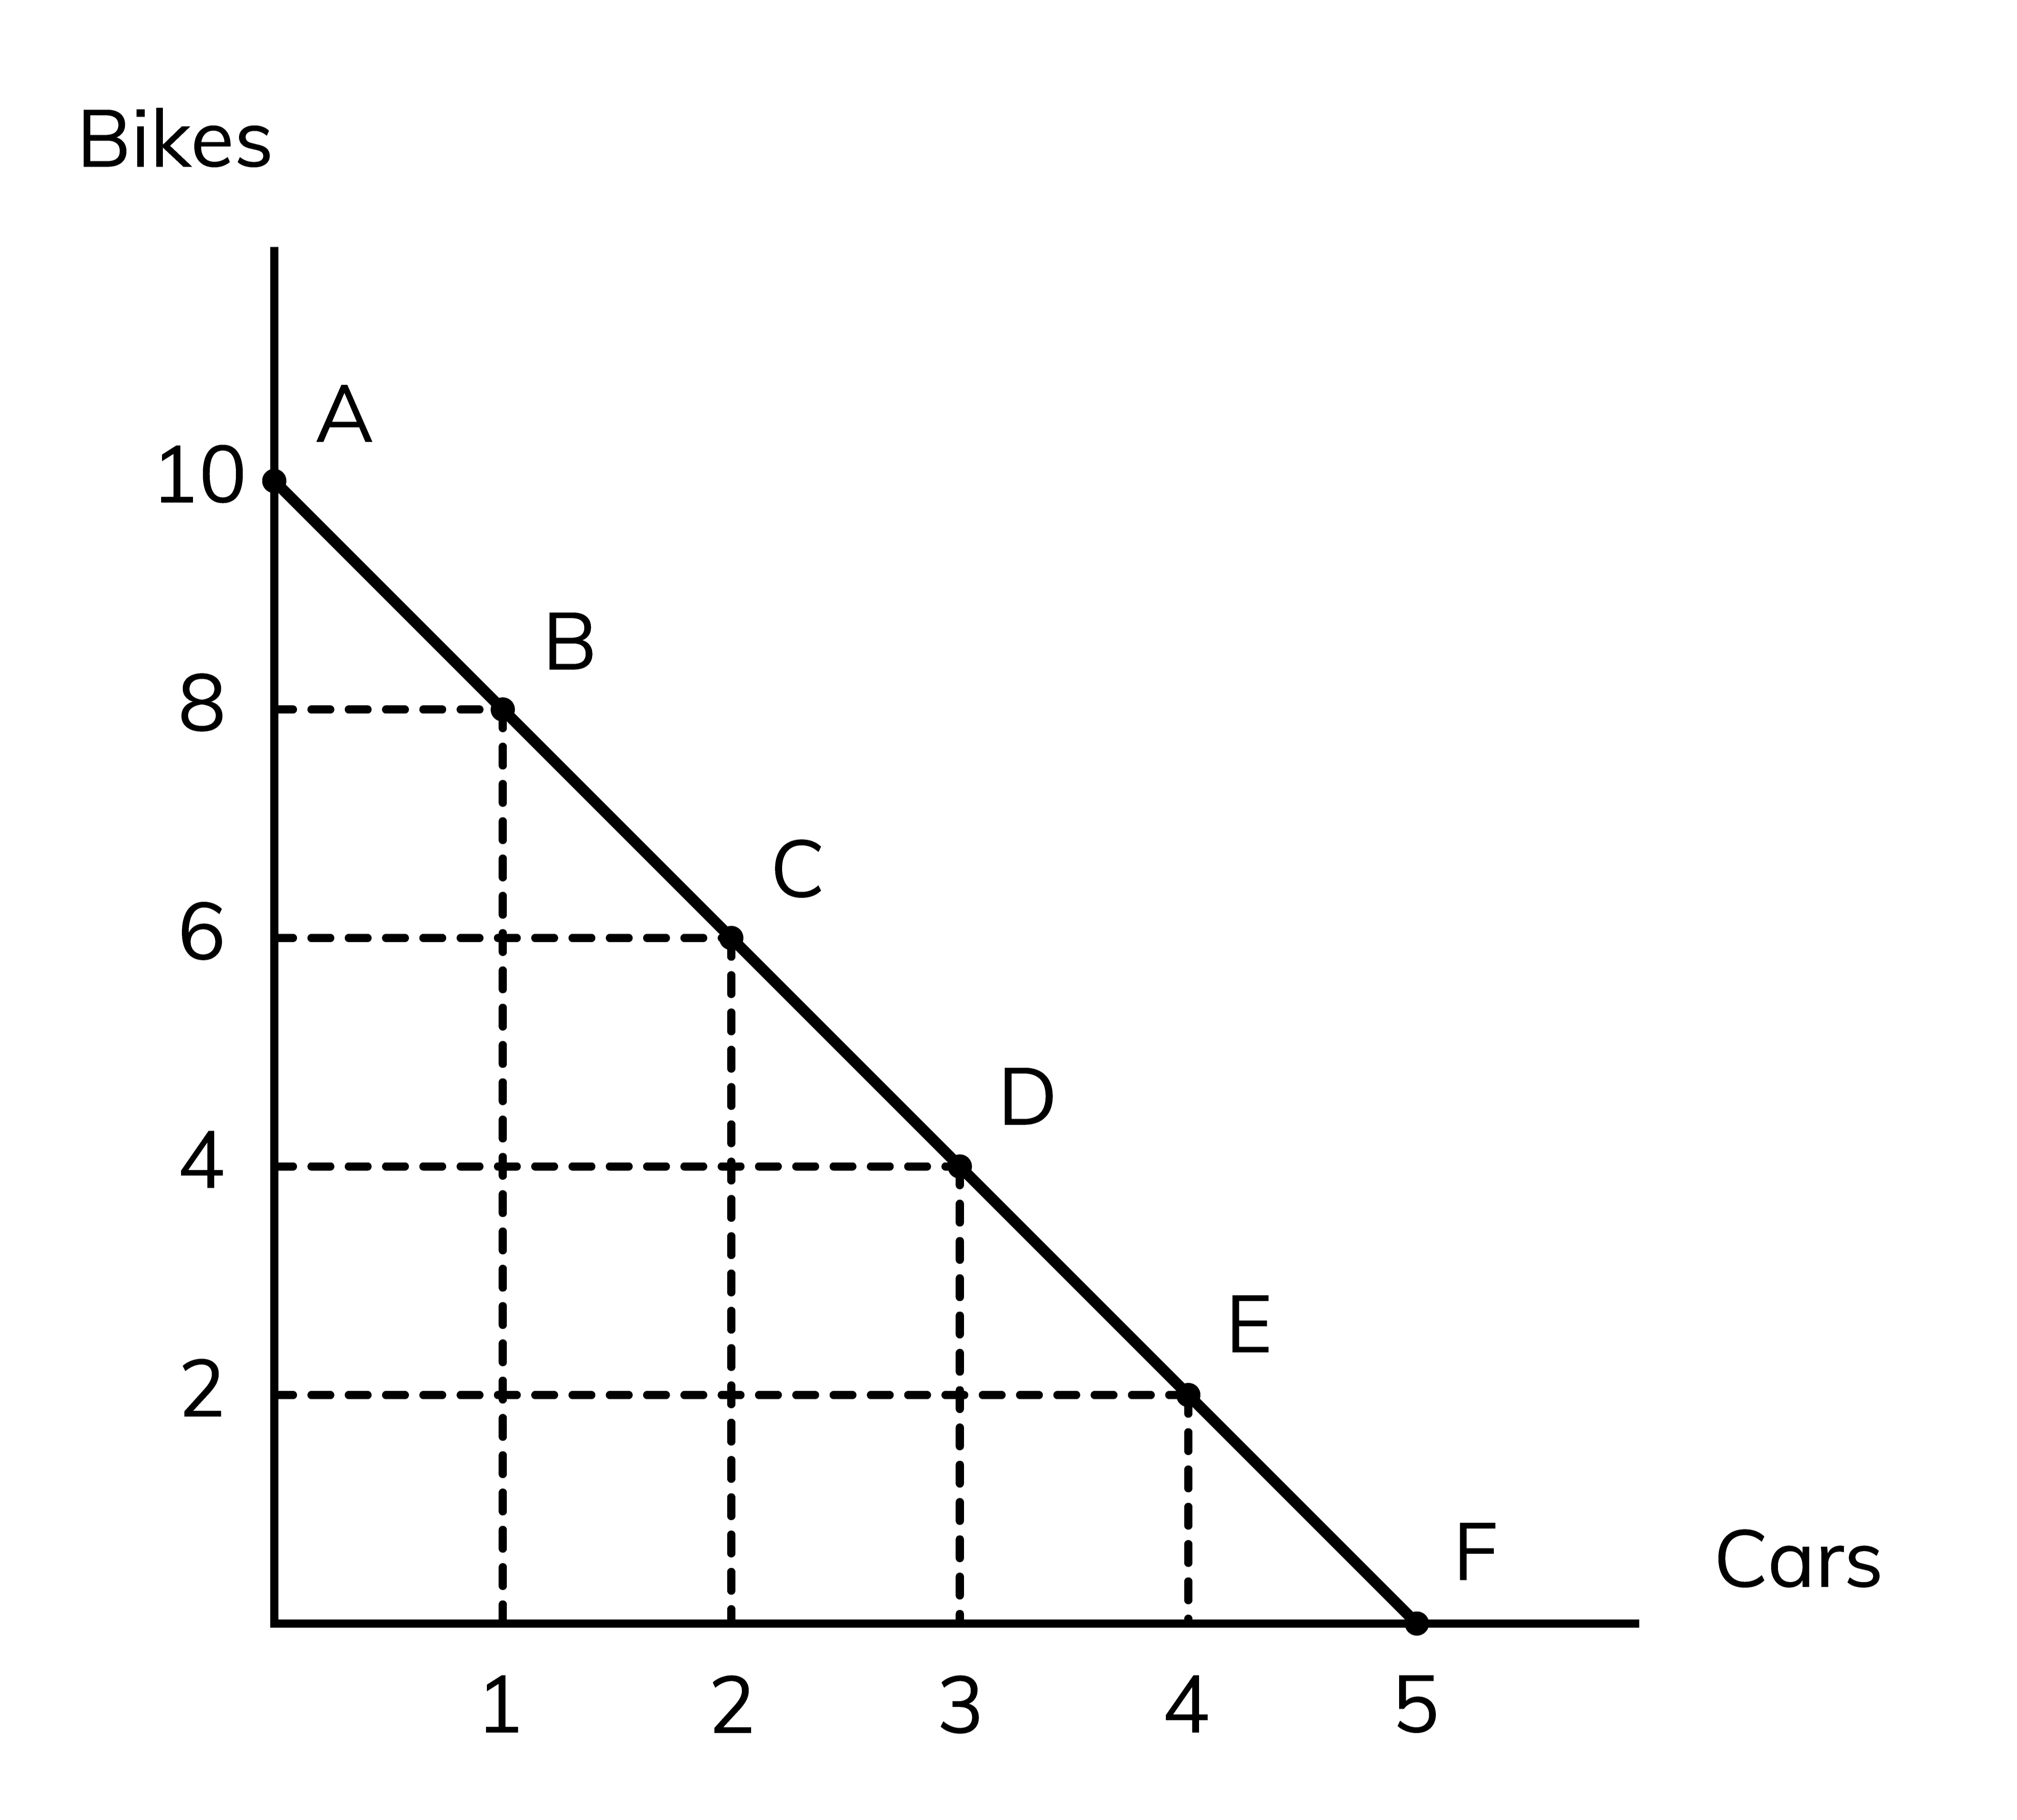
\includegraphics[width=6cm]{linear ppf.png}
\end{center}
\begin{itemize}
    \item What is the slope of the line between A\&F? 
    \item What is the slope of the line between C\&D?
    \item What do these values represent?
\end{itemize}
\end{frame}

\begin{frame}{Interpreting the Slope of a PPF}
\begin{center}
\end{center}
\begin{itemize}[<+>]
    \item The slope of the PPF above represents how much of good $y$ someone has to give up in order to get more of good $x$
    \item This notion is called \textit{opportunity cost}, which is defined in the text as ``what you give up in order to get an item"
    \item In general, the [absolute value of the] slope of a PPF represents the opportunity cost \textit{of good x in terms of y}
    \item Ex: In the above graph, you have to give up 2 ``bikes" to get one ``car" $\iff$ the opportunity cost of 1 car is 2 bikes
\end{itemize}
\end{frame}

\begin{frame}{Slope of a Curved PPF}
\begin{center}
    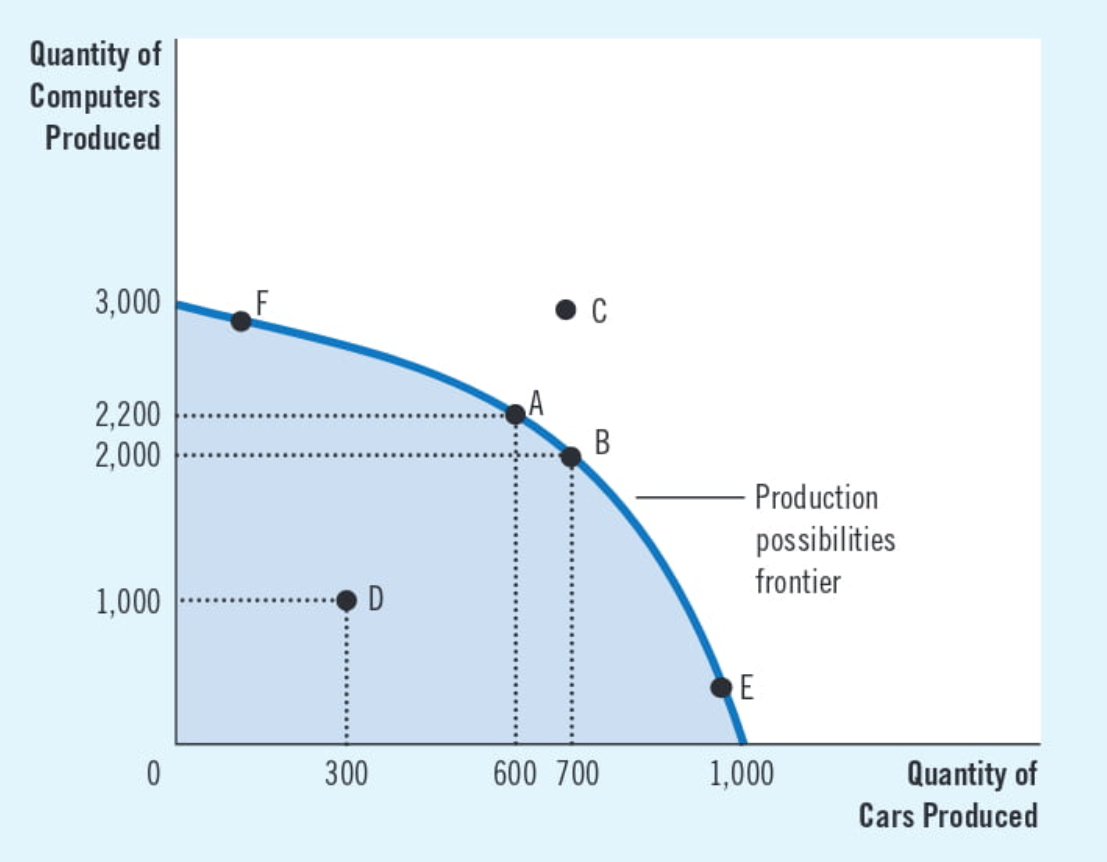
\includegraphics[width=5cm]{ppf from text.png}
\end{center}
\begin{itemize}
    \item You would need calculus to calculate the slope of this graph at any one point, in general
    \item However, we can talk about opportunity cost (OC) moving between two points on this graph:
    \begin{itemize}
        \item The OC of moving from A to B is 200 computers
        \item The OC of moving from E to F ~800 computes\footnote{Note the subtle distinction that the slope of the PPF is the OC of $x$ in terms of $y$, but when we talk about the OC of moving between points, we just report what is given up}
    \end{itemize}
\end{itemize}
\end{frame}

\begin{frame}{One Final Note on Relating OC to the PPF}
\begin{itemize}[<+->]
    \item Note that when we flip the graph from slide 17:\vspace{-1mm}
    \begin{center}
        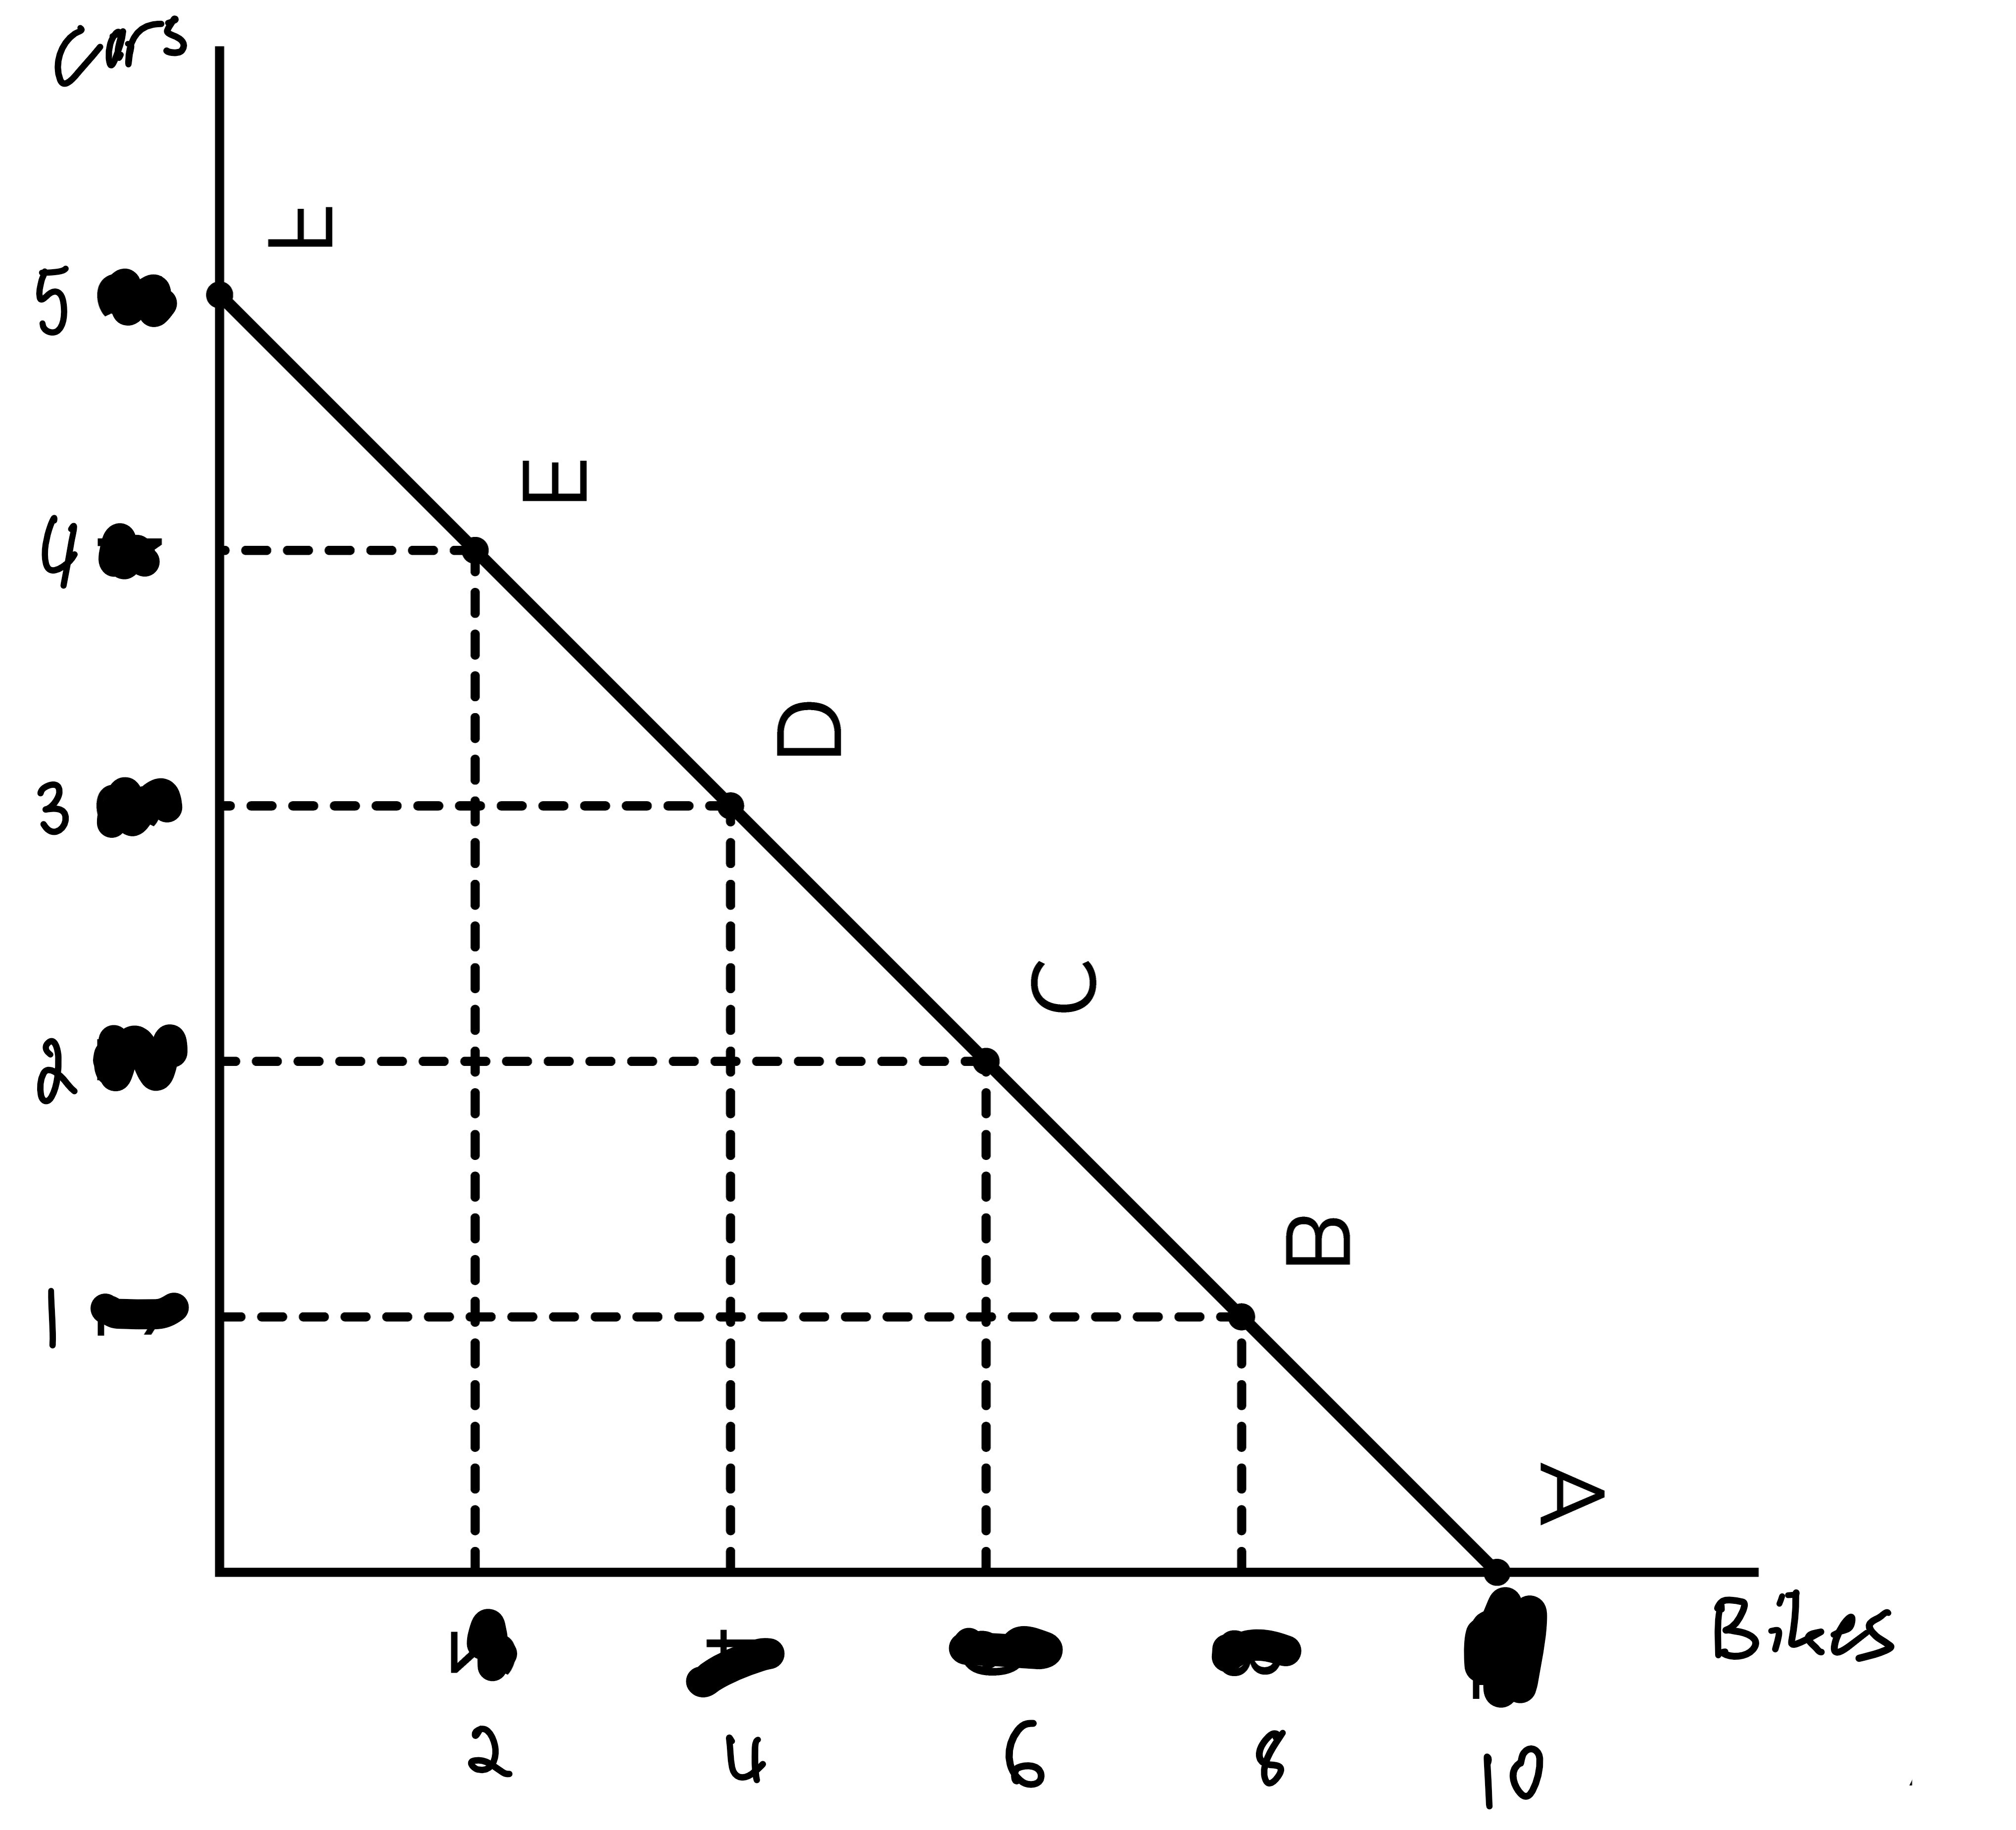
\includegraphics[width=4cm]{linear ppf-rotated.jpg}
    \end{center}
    \vspace{-3mm}
    \item We get that the slope is $-5/10=-\frac{1}{2}$, the inverse (or reciprocal) of what is was last time
    \item This is a key principle: if we give up 2 bikes to get a car, then we give up $\frac{1}{2}$ a car to get a bike
    \item In general: if we give up $a$ units of $x$ to get 1 unit of $y$, then we have to give up $1/a$ units of $y$ if we want 1 unit of $x$
\end{itemize}
\end{frame}

\begin{frame}{Opportunity Cost}
\begin{itemize}[<+->]
    \item A common definition of \underline{\textbf{Opportunity Cost}} is the cost of the \textit{next best thing}
    \item This is an important distinction that earlier definition does not capture
    \item \underline{Ex:} 
    \begin{itemize}
        \item<3-> Your friend invites you to go smoke crack with them later\footnote{Cue all of your friends asking if you do ``all the drugs" now that you live in Oregon}, but you were thinking about studying 
        \item<3-> You were also thinking about going to the gym (but weren't going to do it), and there is a hockey game on in an hour (you do not watch hockey)
        \item<3-> Q: What are you missing out on?
        \item<4-> A: You only miss out on the lost study time, because we all know you aren't going to the gym, and you've literally never turned on hockey before
        \item<5-> That is, the opportunity cost of smoking crack is missed study time
    \end{itemize}
    \item Opportunity cost doesn't count the things that wouldn't have mattered to you
\end{itemize}
\end{frame}



\begin{frame}{OC Example + Math Review}
\begin{itemize}[<+->]
    \item You have \$1000 and are thinking of buying an influencer setup, which gets you nothing but hope for the year
    \item You can buy government bonds and get 0.05\% interest per month
    \item You can throw your money at an ETF or index fund, and make 15\% this year
    \item You can do the smart thing and invest all your money in whatever is trending on WSB this week, yielding you 50\% today, and then -68.9 thereafter\%
    \item Q: What is the total cost of the influencer setup?\vspace{7mm}
    \item A: Direct Cost = \$1000, OC = \$150, so \$1150
\end{itemize}
\end{frame}


\begin{frame}{OC Example 2}
\vspace{-3mm}
\begin{center}
    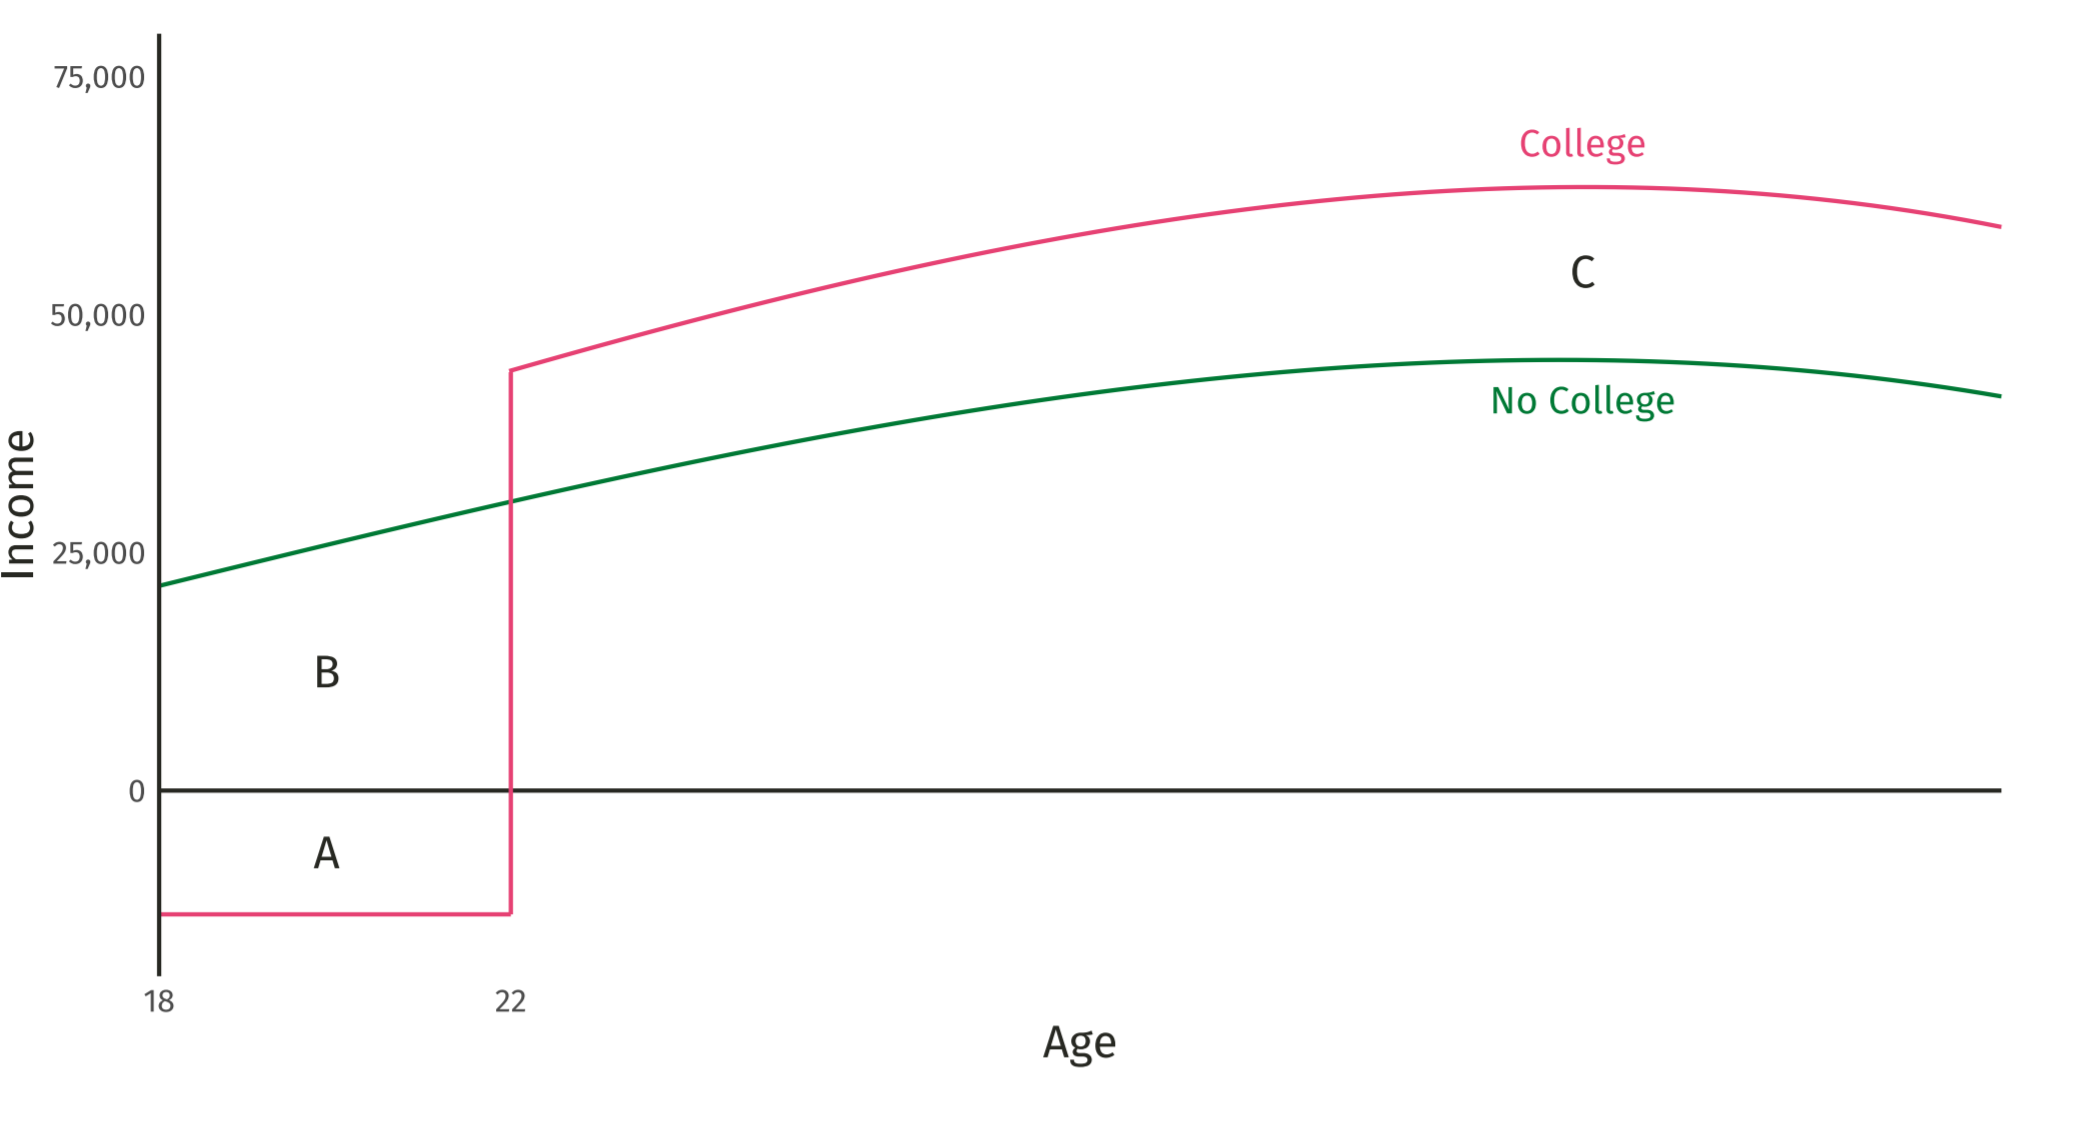
\includegraphics[width=10cm]{college-earnings-profile.png}
\end{center}
\vspace{-5mm}
\begin{itemize}[<+>]
    \item Q: What is the opportunity cost of college?
    \item A: Area B
    \item Notice that A is the \textit{direct cost} of college, while B is the \textit{opportunity cost} of college
\end{itemize}
\end{frame}


\begin{frame}{OC and Trade}
\begin{itemize}[<+->]
    \item Let's consider again a world with two goods: pizza and beer
    \item This time, there are two people in this world: Amay and Britney
    \item Amay can brew 9 gallons of beer (and make 0 pizzas), or he can make 54 pizzas (and brew no beer); Britney can make 13 gallons of beer or make 65 pizzas
    \begin{table}[]
        \centering
        \begin{tabular}{c|c|c|} 
            & Beer & Pizza\\
            \hline
            Amay & 9 & 54 \\
            \hline
            Britney & 13 & 65\\
            \hline
        \end{tabular}
    \end{table}
    \item Note: Whenever you see this sort of table, unless otherwise mentioned, assume OCs are constant (recall the linear PPF)
    \item What is Amay's OC of brewing beer?
\end{itemize}
\end{frame}

\begin{frame}{Amay's PPF}

\end{frame}

\begin{frame}{OC and Trade (cont.)}
    \begin{table}[]
        \centering
        \begin{tabular}{c|c|c|} 
            & Beer & Pizza\\
            \hline
            Amay & 9 & 54 \\
            \hline
            Britney & 13 & 65\\
            \hline
        \end{tabular}
    \end{table}
\begin{itemize}[<+>]
    \item Q: What is Amay's OC of brewing beer?
    \item A: When Amay brews 1 beer, he gives up making 6 pizzas\footnote<2->{\vspace{2mm}Always check that sizes make sense: Amay can make more pizzas than beers, so brewing a beer should cost $>1$ pizza}
    \item Q: What is Britney's OC of brewing beer?
    \item A: Hopefully you can see from the previous example, we can just do $65/13=5$ pizzas. You can visualize this in units as 
    $$\frac{65 \text{ pizza}}{13\text{ beer}}\cdot 1\text{ beer}=\frac{65 \text{ pizza}}{13\cancel{\text{ beer}}}\cdot 1\cancel{\text{ beer}}=5\text{ pizza}$$
\end{itemize}
\end{frame}

\begin{frame}{OC and Trade (Bonus)}
\begin{itemize}[<+>]
    \item Without dividing any of the numbers in the previous table, what are Amay and Britney's OC of making pizza?
    \item 1/6 and 1/5, respectively, since the reciprocal of the OC of $x$ in terms of $y$ gives the OC of $y$ in terms of $x$
\end{itemize}
\end{frame}

\begin{frame}{Should Amay and Britney Take the Next Step?}
\begin{itemize}[<+->]
    \item Should Amay and Britney move in together, and share the goods they produce (trade)?
    \item Britney is better at making both things, would she benefit from living with Amay?
    \item Let's see. Britney, is better at making both things, which we call having an \textit{absolute advantage} in each good 
    \item However, when Amay makes a pizza, he gives up making 1/6 of a gallon of beer; when Britney makes a pizza, she gives up making 1/5 of a gallon of beer
    \begin{itemize}
        \item $\frac{1}{5}>\frac{1}{6}$, so Britney gives up making more beer than Amay does when she chooses to make a pizza
    \end{itemize}
    \item Likewise, Amay forgoes 6 pizzas upon making a beer, while Britney only forgoes 5; Amay gives up making more pizza than Britney does when he chooses to make beer
    \item Put another way, Amay has a \underline{lower OC for pizza}, while Britney has a \underline{lower OC of beer}
    \item As economists, we say that Amay has the \textit{comparative advantage} in pizza, while Britney has the \textit{comparative advantage} in beer
\end{itemize}
\end{frame}

\begin{frame}{Absolute and Comparative Advantage}
\begin{itemize}[<+->]
    \item \underline{\textbf{Absolute Advantage}} is defined by the book as ``the ability to produce a good using fewer inputs than another producer"
    \item \underline{\textbf{Comparative Advantage}} is defined by the book as ``the ability to produce a good at a lower opportunity cost than another producer"
\end{itemize}
    \underline{A bit of history} 
\begin{itemize}
    \item Adam Smith believed that absolute advantage was the sole principle that should guide trade; he believed that if a country was good at producing everything, it would have no reason to trade with anybody
    \item Years later, David Ricardo showed that a country could be worse at something than another country, but still have a comparative advantage in that good, and that this should be the guiding principle for trade
    \item Over the decades, we got more complex models and examples of this result (see Heckscher-Ohlin Model), and today as economists we know that there are gains from trade, specifically from specialization
\end{itemize}
\end{frame}

\begin{frame}{Should Steph Curry be His Own Secretary?}
\begin{itemize}[<+->]
    \item Suppose Steph Curry, through the dexterity it takes to be a bro basketball player, develops a tying speed that's 2x the average professional secretary. Q: Should he do all of his documents himself?
    \item Suppose it costs Steph \$80,000 to hire a secretary, who does 2000 hours of work per year (\$40/hr)
    \item However, Steph normally makes \$1,000,000/hour or more while working (playing basketball)
    \item Even if he had to find other basketball-related work to do, he could probably make in the \$10,000s  of dollars an hours range. 
    \item So, should Steph spend 2000 as a secretary because he's good at it, or should he hire someone?
    \item A: Steph should being doing basketball- or celebrity related work, and hire a secretary for the lower cost
\end{itemize}
\end{frame}


\begin{frame}{Should Amay and Britney Move in Together?}
    \begin{table}[]
        \centering
        \begin{tabular}{c|c|c|} 
            & Beer & Pizza\\
            \hline
            Amay & 9 & 54 \\
            \hline
            Britney & 13 & 65\\
            \hline
        \end{tabular}
    \end{table}
\begin{itemize}[<+->]
    \item Recall that inside the PPF is inefficient, and being on a PPF is efficient
    \item What is are Amay and Britney's individual PPFs? Their combined PPFs?
    \item Their individual PPFs are:\vspace{50mm}
\end{itemize}
\end{frame}

\begin{frame}{Their combined PPF\footnote{This gives a rough description of the construction on the next slide}}
\begin{itemize}[<+->]
    \item Suppose both parties specialized in the good they have a comparative advantage in. Consider this as the starting point for a PPF
    \item If we suppose the Amay specializes and Britney deviates to making both pizza and beer, we obtain Britney's individual PPF, starting from the specialization point
    \item If we suppose instead that Britney specializes and Amay deviates, then we get Amay's individual PPF, connecting to the specialization point
    \item Note that inside the combined PPF is inefficient, while at least one party should specialize in order to achieve efficiency. This includes the point where the two parties specialize in the goods which they \textit{do not} have the comparative advantage
\end{itemize}
\end{frame}

\begin{frame}{Their combined PPF Graph}

\end{frame}

\begin{frame}{Should Countries Trade?}
\begin{itemize}[<+->]
    \item Suppose the U.S. is good at producing lumber, steel, tires, etc., better than any other country
    \item Should the U.S. keep all of it's production at home, and never trade? What if the U.S. was worse at some things?
\end{itemize}
\end{frame}

\begin{frame}{Extra Slide}

\end{frame}

\begin{frame}{Extra Slide}

\end{frame}

\begin{frame}{Extra Slide}

\end{frame}

\begin{frame}{Extra Slide}

\end{frame}

\begin{frame}{Extra Slide}

\end{frame}








\end{document}